\chapter{Marco Teórico}

 En este capitulo se aborda el marco teórico necesario para comprender mas fácilmente el desarrollo de los capítulos posteriores. Se analiza el problema del trafico en general, los simuladores y la teoría detrás del algoritmo a utilizar.

\subsection{Problema del transito vehicular}

En gran parte del mundo se esta produciendo un crecimiento sostenido del parque automotor lo que ocasiona una serie de problemas que afectan la calidad de vida de las personas relacionados con el agravamiento de las congestiones vehiculares \citep{Cepal2003}.

Este problema tiene un gran impacto en el desarrollo de las ciudades por lo que es un componente principal en los planes estratégicos para su crecimiento.

La congestión ocasiona una progresiva merma en la velocidad promedio de circulación, lo que incrementa la duración de los viajes, aumenta el consumo de combustible y la contaminación atmosférica y sonora, lo que repercute directamente en la salud de las personas. 
Ademas se genera una exigencia en las vías de transito que ocasiona un deterioro mayor de calles y rutas.

Uruguay no escapa a este fenómeno en particular Montevideo, donde el aumento del parque automotor esta en ascenso constante desde el 2005 \citep{INE2014} 
Y según proyecciones el crecimiento seguiría en un promedio de 4.5\% anual hasta el 2020. \citep{BBVA2013}

Esto viene de la mano con el sostenido aumento de las ventas de vehículos  desde el 2003 \citep{Autoanuario2014}

Los expertos indican que la congestión ya esta instalada y la infraestructura vial no acompaso este crecimiento. Ademas se indica que Montevideo es la ciudad con mas semáforos por automóvil en Latinoamerica. Con mas de 620 cruces semaforizados, alguno de los cuales no están coordinados.\citep{Subrayado2013}

Por todo esto es relevante el tema de la sincronización de semáforos para agilizar el transito y no generar congestiones, aumentando la velocidad promedio de los viajes y mejorando las perspectivas de desarrollo de la ciudad así como la calidad de vida de sus habitantes.

\subsection{Corredor Garzón}
El corredor Garzón esta ubicado en Montevideo Uruguay, fue construido como parte de un plan de movilidad que incluye otros 4 corredores. 
Presenta un carril exclusivo para ómnibus y preferenciales
http://www.montevideo.gub.uy/ciudadania/stm-transporte-metropolitano/plan-de-movilidad/corredores

Tiene 6km de largo , extendiéndose desde ...  hasta ..
%http://www.montevideo.gub.uy/sites/default/files/articulo/corredor_garzon.pdf

Agregar mapa y poner referencia de donde se saco

Los problemas de sincronización de semáforos fueron admitidos en varias publicaciones.

18 diciembre 2013 - Corredor Garzón lucha contra el tiempo %http://www.elpais.com.uy/informacion/imm-corredor-garzon-tiempos-cambios.html
Dice que antes de Garzon se demoraba promedio 18 minutos, y al inaugurar el corredor 30 minutos. Después se mejoro algo para equilibrar los tiempos
Para el jerarca, eso se dio "con la diferencia de que hoy hay 15 semáforos más y se ganó en seguridad". En concreto, tras la obra, se pasó de tener 5 semáforos a 20. Según Campal, su des-coordinación inicial, entre otros aspectos, fue lo que provocó tales demoras, generando malestar en los usuarios.
inversión de 60 millones


4 agosto 2013 - Garzon desde un omnibus %http://www.elpais.com.uy/informacion/corredor-garzon-visto-bus.html


30 julio 2013  - Intendetnta admite errores %http://www.elpais.com.uy/informacion/garzon-olivera-admitio-errores.html
La intendenta admte errores y dice: no se ha logrado sincronizar los semáforos. Hay un tema con el software,(y) la empresa subcontratada no ha dado los resultados esperados


Abril 2013 - Otro Corredor con obras paralizadas por criticas a GArzon
%http://www.elpais.com.uy/informacion/marcha-atras-en-corredor-agraciada.html






\section{Simulación y herramientas}

\subsection{Simuladores de tráfico}
Los simuladores de tráfico son programas que simulan el movimiento de vehículos sobre una red de calles, es una herramienta muy usada en la investigación de trafico vehicular, así como estudio de congestiones o análisis de impacto que tendrán nuevas infraestructuras.  Las razones para usar una simulación son varias, entre ellas se encuentra  la rapidez, ya que la simulación se puede realizar en tiempo mucho mas rápidos que en la realidad, el costo en dinero ya que no estamos afectando el escenario real  y tampoco tenemos que modificar o detener el escenario real para probar nuevos parámetros. Ademas nos sirve para poder prever situaciones que podrían darse bajo determinadas circunstancias.

Los simuladores se pueden dividir en microscópicos o macroscópicos según el nivel de detalle de la simulación. Un simulador macroscópico modela  el trafico vehicular como un fluido. En cambio un simulador microscópico simula el movimiento de cada vehículo según sus características particulares.

SUMO\citep{SUMO} es uno de los simuladores abiertos mas populares, es microscópico y utiliza una serie de archivos  XML que representan las rutas, los vehículos y el trafico.  

Cuanto mas crece el numero de vehículos y la complejidad de la red de mapas mas difícil se hace crear la entrada básica que necesita el simulador. Aunque existen diversas herramientas que ayudan a este proceso aun se requiere un trabajo manual para el acondicionado de estos archivos.

En las siguientes secciones se muestra mas en detalle algunas de sus funcionalidades y características.


\subsection{Modelo de trafico }
Esta es la representación de la circulación de vehículos, aquí exponemos algunos de los mas populares. 

Aleatorios: Genera diferentes recorridos que seguirán los vehículos aleatoriamente

JTR (junction turning ratio) : basados en probabilidades en los cruces  es decir cuando un vehículo llega a un cruce tiene cierta probabilidad de seguir o doblar.
 
Basado en áreas:  Se especifican áreas como un conjunto de calles y se realizan recorridos entre ellas.


Basado en Actividad: Se especifica la cantidad de casas, vehículos y población en un determinado lugar y el modelo genera la densidad de trafico que se producirá basado en los tipos de actividades que se realizan comúnmente como ir al trabajo, hacer las compras, ir a la escuela,  etc

Definido por el usuario: que permiten determinar la ruta de los vehículos con mayor detalle.

\subsection{Representaciones}

\subsubsection{Red de calles}
La red de calles se representa como un grafo dirigido en un archivo xml con extensión .net.xml . Allí se especifican los nodos, y vértices así como sus atributos. También se representan los semáforos. Esto  se genera utilizando una herramienta  para convertir un mapa al formato que SUMO utiliza.

\subsubsection{Representación Trafico}
En este caso también se utiliza un archivo xml donde se definen las rutas y los recorridos. Un recorrido representa el movimiento de un vehículo de un punto inicial hacia un punto final (El recorrido se hacen en tiempo de ejecución utilizando el camino mas corto basado en el trafico). 


\subsubsection{Representación del tiempo}
El tiempo se representa como una serie de pasos discretos, cada uno durando un segundo. Este valor se puede modificar aunque es recomendado dejarlo así para que sea consistente.


\subsubsection{Tipos de vehículos}
Se pueden crear diferentes tipos de vehículos especificando propiedades como largo, velocidad máxima,  aceleración, color, etc. También cuenta con vehículos por defecto como buses, camiones o automoviles.







\subsection{Configuración de la simulación}

En esta sección se realiza un resumen sobre los pasos realizados para tener los elementos necesarios para realizar la simulación.

\subsubsection{Diseño del mapa}


El mapa base de la zona proviene de Open Street Map \citep{OSM}, luego se cotejo su exactitud con Google Maps y Bing Maps.

\begin{figure}[h]
\centering
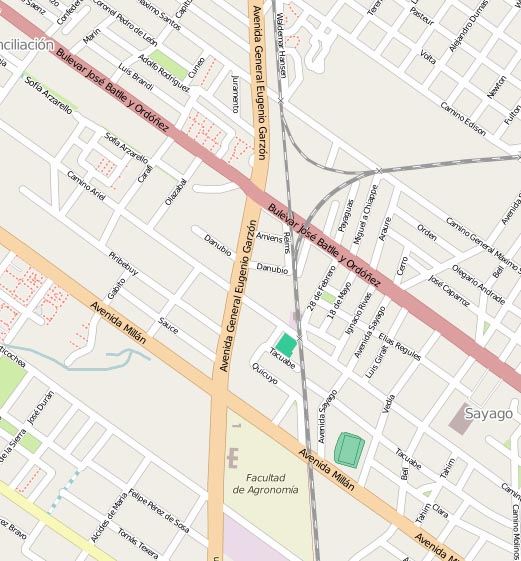
\includegraphics[width=0.7\linewidth]{Figures/osm_garzon}
\caption{Tramo del mapa de Garzon de OSM}
\label{fig:osm_garzon}
\end{figure}


Se utilizo la herramienta netconvert para convertirlo al formato que SUMO acepta. 
Para esto se realizaron varios ajustes editando los archivos xml para corregir errores en las calles, cruces y conexiones para que fuese fiel a la realidad y mantuviera la compatibilidad con SUMO.


\begin{figure}[h]
\centering
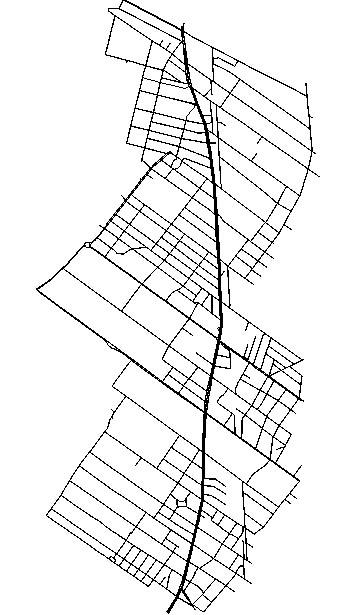
\includegraphics[width=0.5\linewidth]{Figures/mapa_sumo}
\caption{Mapa cargado en SUMO luego del modelado y procesamiento}
\label{fig:mapa_sumo}
\end{figure}



\subsubsection{Trabajo de campo realizado}
Al no contar con datos públicos sobre la configuración de los semáforos de la zona, realizamos un revelamiento in-situ con las siguientes características.

Se seleccionaron 5 cruces que presentan diferentes características para poder modelar las variantes tanto de cruces con alto trafico, medio y bajo. 
Estos son: Camino Ariel, Battle y Ordoñez, Plaza Videla, Camino Colman y Aparicio Saravia.

Se eligió el día miércoles, que estuviera soleado y entre las 15 y 17 horas para no tener los sesgos que se producen los fines de semana o días de lluvia.
Se realizaron filmaciones de 30 min en los cruces y luego se analizaron los vídeos para realizar el conteo manual con la posibilidad de enlentecer el vídeo para mayor facilidad. Luego se completa una planilla excel donde se tiene la información de vehículos que recorren Garzón, la calle que cruza y los que doblan. También discriminamos entre vehículos y ómnibus que recorren Garzón.

\begin{figure}[H]
\centering
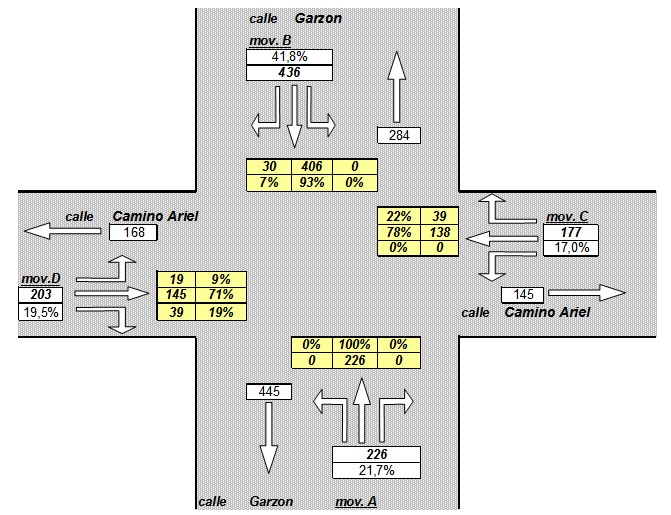
\includegraphics[width=0.7\linewidth]{Figures/conteo_hoja}
\caption{Planilla electrónica para el conteo manual en Camino Ariel}
\label{fig:conteo_hoja}
\end{figure}


Ademas se realizaron recorridas de punta a punta del corredor a una velocidad constante para verificar los tiempos obtenidos en la simulación para este recorrido.

Para obtener la configuración de los semáforos se realizo un recorrido en bicicleta por el corredor cronometrando la duración del tiempo en cada esquina de cada semáforo. Tanto de ida como de vuelta para corroborar que fueran correctos. Estos tiempos fueron verificados por los vídeos obtenidos.


\newpage
\subsubsection{Creación del modelo del trafico}

Con los datos relevados se creo un modelo vehicular de la ciudad [poner el mapa] que brinda una aproximación sobre la densidad de trafico y la velocidad promedio de circulación.

Se utilizo el programa Traffic Modeler \citep{TrafficModeler} con lo que se logra generar modelos de trafico complejo de manera visual y sencilla. Se opto por un modelo de movilidad entre áreas lo que permite una buena granularidad al especificar la densidad de trafico.


\begin{figure}[H]
\centering
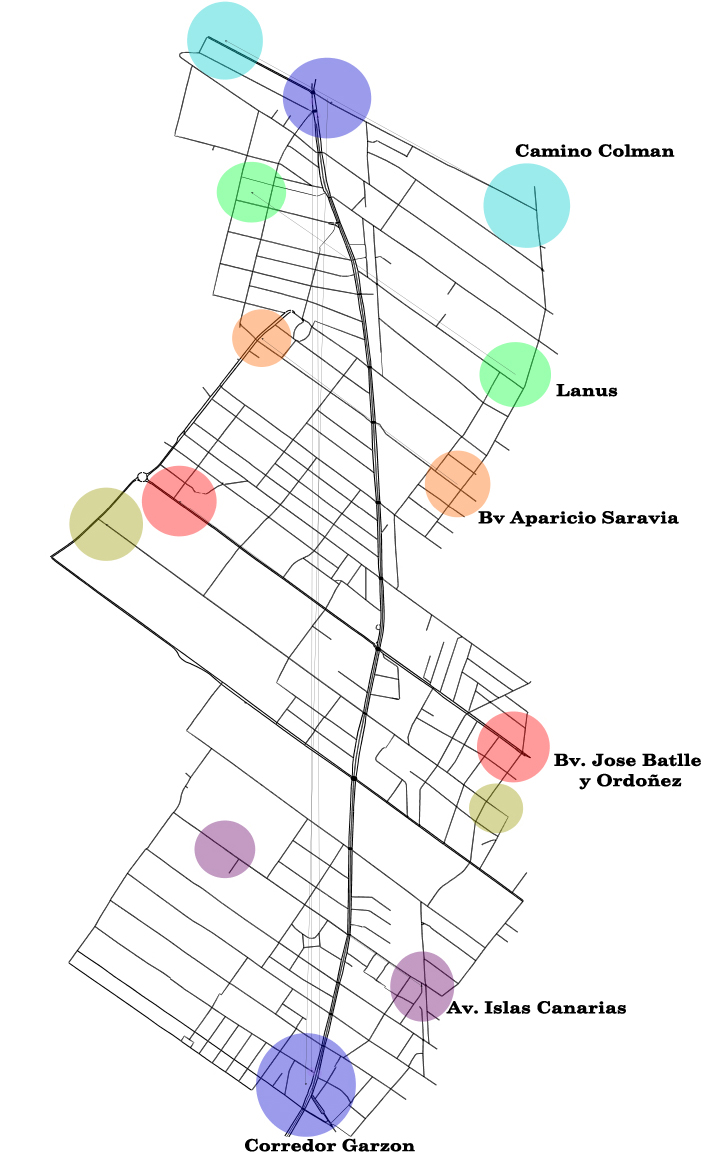
\includegraphics[width=0.4\linewidth]{Figures/areaflow1}
\caption{Mapa del TrafficModeler con las áreas de trafico. Círculos del mismo color indican trafico especificado entre esas áreas}
\label{fig:areaflow1}
\end{figure}


Actualmente no se cuenta con información publica relativa a la configuración de los semáforos en la ciudad, aunque cabe destacar que en el futuro se prevé crear un sistema centralizado de sincronización de semáforos. \citep{OBS01} 
En este caso se agrego la información sobre la configuración de los semáforos de los datos relevados.

Se manejaron dos tipos de vehículos autos y ómnibus cada uno con características distintas tanto de tamaño, aceleración y velocidad máxima.

Se agregaron las frecuencias y los distintos recorridos de los ómnibus obtenidos de datos públicos de la Intendencia de Montevideo \citep{IMM}
Estos incluyen las lineas urbanas  'G',  la  '409' , '522'  y  '148' . Las líneas de ómnibus suburbanas realizan  un mismo  trayecto y las generalizamos con el nombre 'A'.  
Todas  las  líneas  de  ómnibus
fueron cargadas con las paradas correspondientes y se
hicieron  variantes  en  los  viajes  dentro  de  una  misma
línea para simular el hecho de que no siempre se para en las mismas paradas.




\begin{figure}[H]
	\centering
	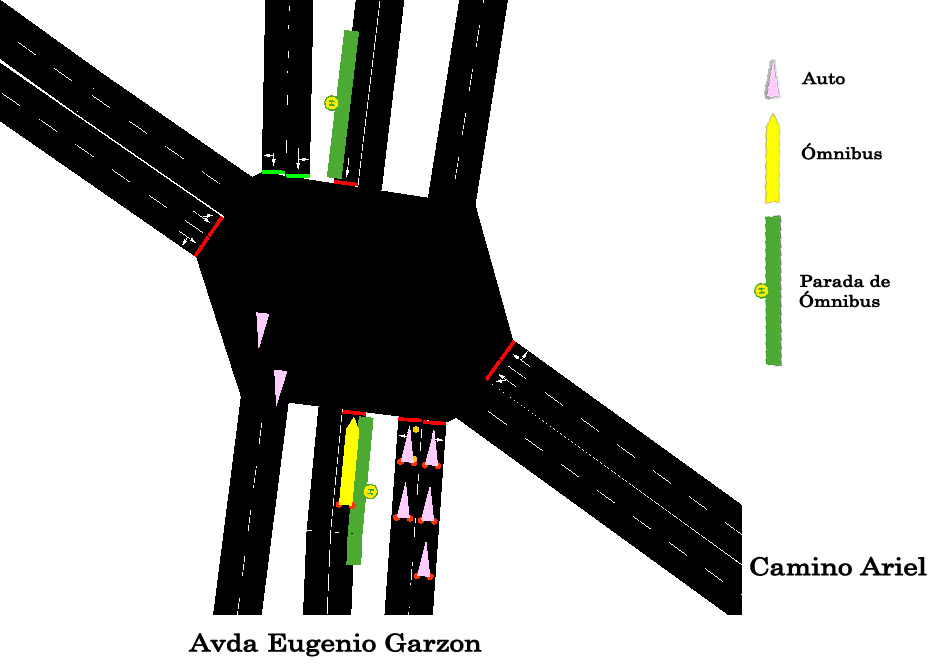
\includegraphics[width=0.7\linewidth]{Figures/sim1}
	\caption{Simulacion de trafico en SUMO en el curce entre Bulevar Battle y Ordoñez y el Corredor Garzon.}
	\label{fig:sim1}
\end{figure}




\section{Herramientas}
Aquí se muestra información útil sobre las herramientas utilizadas.

\subsection{Open Street Map:} 
 Es un proyecto en donde una comunidad crea mapas libres y editables \citep{OSM}. Cuenta con cerca de 1.8 millones de usuarios  y  mas de 20.000 que editaron algo en el ultimo mes \citep{OSMSTATS} por lo que es muy activa. Se utilizan datos de GPS móviles, fotografías satelitales y otras fuentes libres para crear los mapas y editarlos. 

\subsection{SUMO ( Simulation of Urban MObility)}

Es un simulador de trafico gratis y abierto que nos permite modelar redes de calles, vehículos, transporte publico, ciudadanos y semáforos \citep{SUMO}. Sigue un modelo microscópico ya que realiza la simulación individual explicita de cada elemento. Ademas incluye un conjunto de herramientas destinadas  a facilitar la generación de trafico, construcción de mapas, etc. 


\subsection{Por que usar SUMO? }
otras alternativas? Revisar estado del arte?
Sumo es gratis
Nos permite utilizarlo sin interfaz gráfica por linea de comando lo que aumenta sensiblemente la velocidad ed ejecución, y  nos permite visualizar la interfaz gráfica una vez completada la optimización para ver exactamente como se comporta el sistema en la simulación.

Sumo presenta varias salidas con información interesante: \citep{SUMOOUT} 
La salida obtenemos el tiempo de simulación, la cantidad de emitidos y la cantidad de completados. Buscamos que sea > 80%
Permite la ejecución tanto por linea de comando como una interfaz gráfica para visualizar

\subsection{NetConvert}
Utilizado para la generación de la red a partir de un mapa. Por ejemplo podemos transformar un mapa de Open Street Map en archivo XML de red que SUMO reconoce. Este programa viene integrado con SUMO

\subsection{DUaRouter}
 Genera recorridos de vehículos basado en dinámicas definidas por el usuario. Esta utilidad viene integrada con SUMO.

\subsection{Traffic Modeler}
Herramienta para la generación de trafico de manera visual y luego transformarlo para que sea reconocido por SUMO. \citep{TrafficModeler}

\subsubsection{Escenarios}



